\chapter{System Implementation} \label{chap:sysImplementation}
%\version{v1.10.2015}

\section*{}
In this chapter there is system implementation, its technical specifications, algorithms and software components.

\section{System Architecture}
Describe the architecture e.g. in terms of System internal components, Functionality of the components, Communication between the components
ADD system have no physical components. Internally system have different Forms and classes which are linked with each others. These classes perform different functionality and having  XML parsing and join algorithms. These functions are linked with different forms.

\section{Tools and Technology Used}
ADD is basically implemented on Microsoft Visual Studio 2013. Visual Studio provides developer tools and services for any platform and any programming language. Its first version is developed in 1997 by Microsoft. ADD application is implemented in version 2013 shown in Figure \ref{fig:Visual Studio 2013}. 
\begin{figure}[ht]
\centering
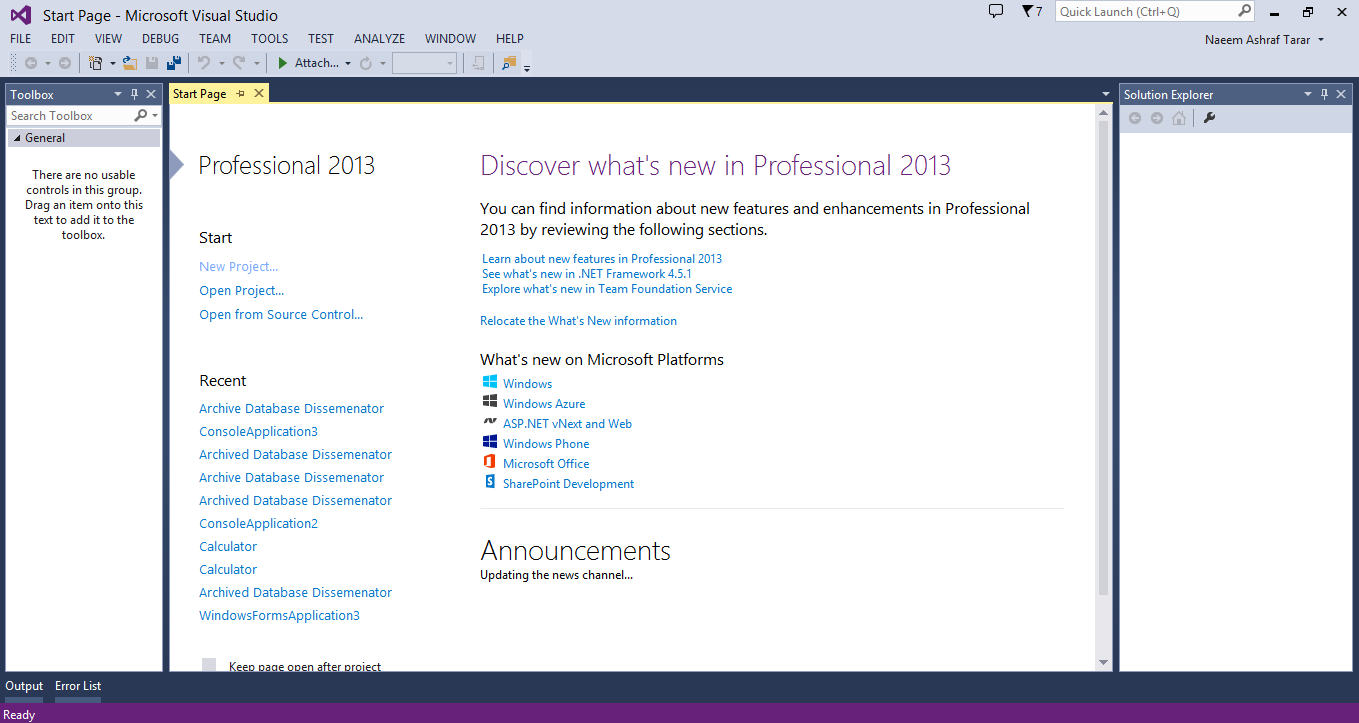
\includegraphics[scale=0.4]{ToolUsed}
\caption{Visual Studio 2013}
\label{fig:Visual Studio 2013}
\end{figure} 
It is compatible with Windows XP, 7, 8 (32/64 – Bit OS). The technique use in ADD application is XML parsing, joining algorithms, sorting and filtering.
\begin{itemize}
	\item Libraries Used: There are many built-in functions and API's used in ADD implementation.
	
	\begin{enumerate}
		\item System.IO.Compression
		\item XmlNamespaceManager
		\item XmlDocument 
	\end{enumerate}
\end{itemize}
 

\section{Development Environment/Languages Used}
\begin{figure}[ht]
\centering
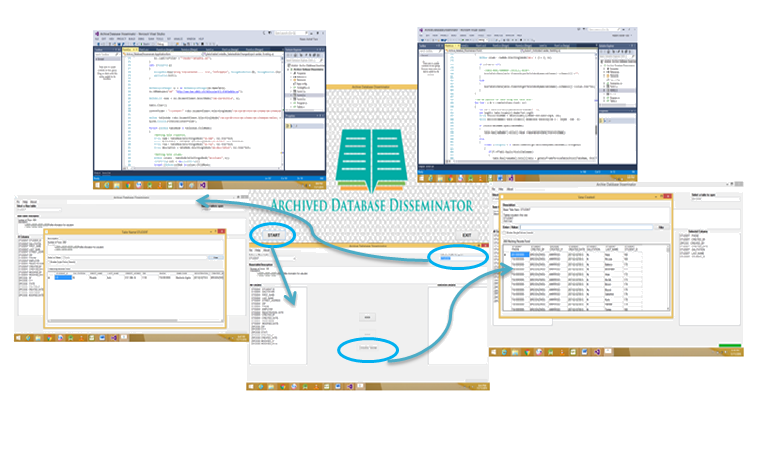
\includegraphics[scale=0.5]{Working}
\caption{ADD Interfaces}
\label{fig:ADD Interfaces}
\end{figure}
Figure \ref{fig:ADD Interfaces} shows detailed working of ADD application. It gets file and work on selected file using C\# Windows Form Application. 

\par There is complete running screen shots of ADD application. How application is start and which interfaces displays after running. How user interact with ADD and which operations and how perform desired operations. How user load the file, view tables, keys, columns, records and at which interface user do filtering and sorting.

\section{Processing Logic/Algorithms}
ADD is basically perform work on archive ".siard" file which is compressed in ".siard" XML format by SIARD tool. ADD load this ".siard" file and parse that XML file for read it. When file is loaded it displays all tables in selected database and also its keys. Select specific table displays its columns and can view complete table's record. Using join algorithms it make a view of selected columns and displays the newly created view. Using filter user can search specific record and can sort the record \cite{code}. 

\section{Application Access Security}
ADD application runs on windows system. It has no connection with databases so it can not disturb database. ADD is not encrypt or decrypt any data. No need of installation it directly runs on system. ADD have no link with firewall or other windows security systems. 


 
